\documentclass{beamer}
\mode<presentation>
\usepackage{amsmath}
\usepackage{amssymb}
\usepackage{bm}
\usepackage{adjustbox}
\usepackage{subcaption}
\usepackage{enumerate}
\usepackage{multicol}
\usepackage{mathtools}
\usepackage{listings}
\usepackage{url}
\def\UrlBreaks{\do\/\do-}
\usetheme{Boadilla}
\usecolortheme{lily}
\setbeamertemplate{footline}
{
  \leavevmode%
  \hbox{%
  \begin{beamercolorbox}[wd=\paperwidth,ht=2.25ex,dp=1ex,right]{author in head/foot}%
    \insertframenumber{} / \inserttotalframenumber\hspace*{2ex} 
  \end{beamercolorbox}}%
  \vskip0pt%
}
\setbeamertemplate{navigation symbols}{}

\providecommand{\nCr}[2]{\,^{#1}C_{#2}}
\providecommand{\nPr}[2]{\,^{#1}P_{#2}}
\providecommand{\mbf}{\mathbf}
\providecommand{\pr}[1]{\ensuremath{\Pr\left(#1\right)}}
\providecommand{\qfunc}[1]{\ensuremath{Q\left(#1\right)}}
\providecommand{\sbrak}[1]{\ensuremath{{}\left[#1\right]}}
\providecommand{\lsbrak}[1]{\ensuremath{{}\left[#1\right.}}
\providecommand{\rsbrak}[1]{\ensuremath{\left.#1\right]}}
\providecommand{\brak}[1]{\ensuremath{\left(#1\right)}}
\providecommand{\lbrak}[1]{\ensuremath{\left(#1\right.}}
\providecommand{\rbrak}[1]{\ensuremath{\left.#1\right)}}
\providecommand{\cbrak}[1]{\ensuremath{\left\{#1\right\}}}
\providecommand{\lcbrak}[1]{\ensuremath{\left\{#1\right.}}
\providecommand{\rcbrak}[1]{\ensuremath{\left.#1\right\}}}
\providecommand{\rank}{\text{rank}}
\theoremstyle{remark}
\newtheorem{rem}{Remark}
\newcommand{\sgn}{\mathop{\mathrm{sgn}}}
\providecommand{\abs}[1]{\ensuremath{\left\vert #1 \right\vert}}
\providecommand{\res}[1]{\Res\displaylimits_{#1}} 
\providecommand{\norm}[1]{\lVert#1\rVert}
\providecommand{\mtx}[1]{\mathbf{#1}}
\providecommand{\mean}[1]{\overline{#1}}
\providecommand{\fourier}{\overset{\mathcal{F}}{ \rightleftharpoons}}
\providecommand{\system}{\overset{\mathcal{H}}{ \longleftrightarrow}}
\providecommand{\dec}[2]{\ensuremath{\overset{#1}{\underset{#2}{\gtrless}}}}

% this \vec is already defined in your file:
\renewcommand{\vec}[1]{\begin{pmatrix}#1\end{pmatrix}}

\newenvironment{amatrix}[1]{%
  \left(\begin{array}{@{}*{#1}{c}|c@{}}
}{%
  \end{array}\right)
}

\lstset{
frame=single, 
breaklines=true,
columns=fullflexible
}
\usepackage{listings}
\lstset{
  language=Python,
  basicstyle=\ttfamily\small,
  numbers=left,
  numberstyle=\tiny,
  breaklines=true,
  frame=single
}

\title{Matgeo-4.8.15}
\author{AI25BTECH11019-Menavath Sai Sanjana}

\date{}

\begin{document}
  
\begin{frame}  
\titlepage  
\end{frame}  
   

\begin{frame}  
\frametitle{Question}  
A line $l$ passes through point $(-1,3,-2)$ and is perpendicular to both the lines  
$\frac{x-1}{1} = \frac{y-1}{2} = \frac{z+1}{3}$ and  
$\frac{x+2}{-3} = \frac{y}{2} = \frac{z}{5}$. Find the vector equation of the line $l$ and its distance from the origin.  
\end{frame}  

\begin{frame}
\frametitle{Question}
A line $l$ passes through $(-1,3,-2)$ and is perpendicular to both the lines  
\begin{align}
\frac{x-1}{1} = \frac{y-1}{2} = \frac{z+1}{3}, \quad
\frac{x+2}{-3} = \frac{y}{2} = \frac{z}{5}.
\end{align}
Find the vector equation of $l$ and its distance from the origin.
\end{frame}

\begin{frame}
\frametitle{Solution}

The two given direction vectors are
\begin{align}
\vec{d}_1 = \vec{1\\2\\3}, \quad 
\vec{d}_2 = \vec{-3\\2\\5}.
\end{align}

Let the required direction vector be $\vec{u}=\vec{u_1\\u_2\\u_3}$.
It satisfies
\begin{align}
\vec{d}_1^\top \vec{u} &= 0, \\
\vec{d}_2^\top \vec{u} &= 0.
\end{align}
\end{frame}

\begin{frame}
\frametitle{Solution}

Substituting values,
\begin{align}
u_1 + 2u_2 + 3u_3 &= 0, \\
-3u_1 + 2u_2 + 5u_3 &= 0.
\end{align}

Eliminating $u_1$:
\begin{align}
8u_2 + 14u_3 &= 0 \;\;\Rightarrow\;\; u_2 = -\frac{7}{4}u_3.
\end{align}

Substitute in the first equation:
\begin{align}
u_1 + 2\left(-\frac{7}{4}u_3\right) + 3u_3 = 0
\;\;\Rightarrow\;\; u_1 = \frac{1}{2}u_3.
\end{align}
\end{frame}

\begin{frame}
\frametitle{Solution}

Choosing $u_3=4$ gives integer values:
\begin{align}
\vec{u} = \vec{2\\-7\\4}.
\end{align}

Hence the line through $(-1,3,-2)$ is
\begin{align}
\vec{r} = \vec{-1\\3\\-2} + t\,\vec{2\\-7\\4}, \quad t\in\mathbb{R}.
\end{align}
\end{frame}

\begin{frame}
\frametitle{Distance from Origin}

For the closest point, parameter
\begin{align}
t = -\frac{\vec{P}\cdot\vec{u}}{\vec{u}\cdot\vec{u}}
= -\frac{(-1)(2)+3(-7)+(-2)(4)}{2^2+(-7)^2+4^2}
= \frac{31}{69}.
\end{align}

So the foot of the perpendicular is
\begin{align}
\vec{Q} = \vec{P}+t\vec{u} 
= \vec{-\tfrac{7}{69}\\\\ -\tfrac{10}{69}\\\\ -\tfrac{14}{69}}.
\end{align}

Distance:
\begin{align}
D = \|\vec{Q}\| = \sqrt{\frac{5}{69}}.
\end{align}
\end{frame}

\begin{frame}
\frametitle{Conclusion}

The required line is
\begin{align}
\vec{r} = \vec{-1\\3\\-2} + t\,\vec{2\\-7\\4}, \quad t\in\mathbb{R},
\end{align}
and the distance from the origin is
\begin{align}
D = \sqrt{\frac{5}{69}}.
\end{align}
\end{frame}

\begin{frame}
\frametitle{Graphical Representation}

\begin{figure}[ht!]
    \centering
    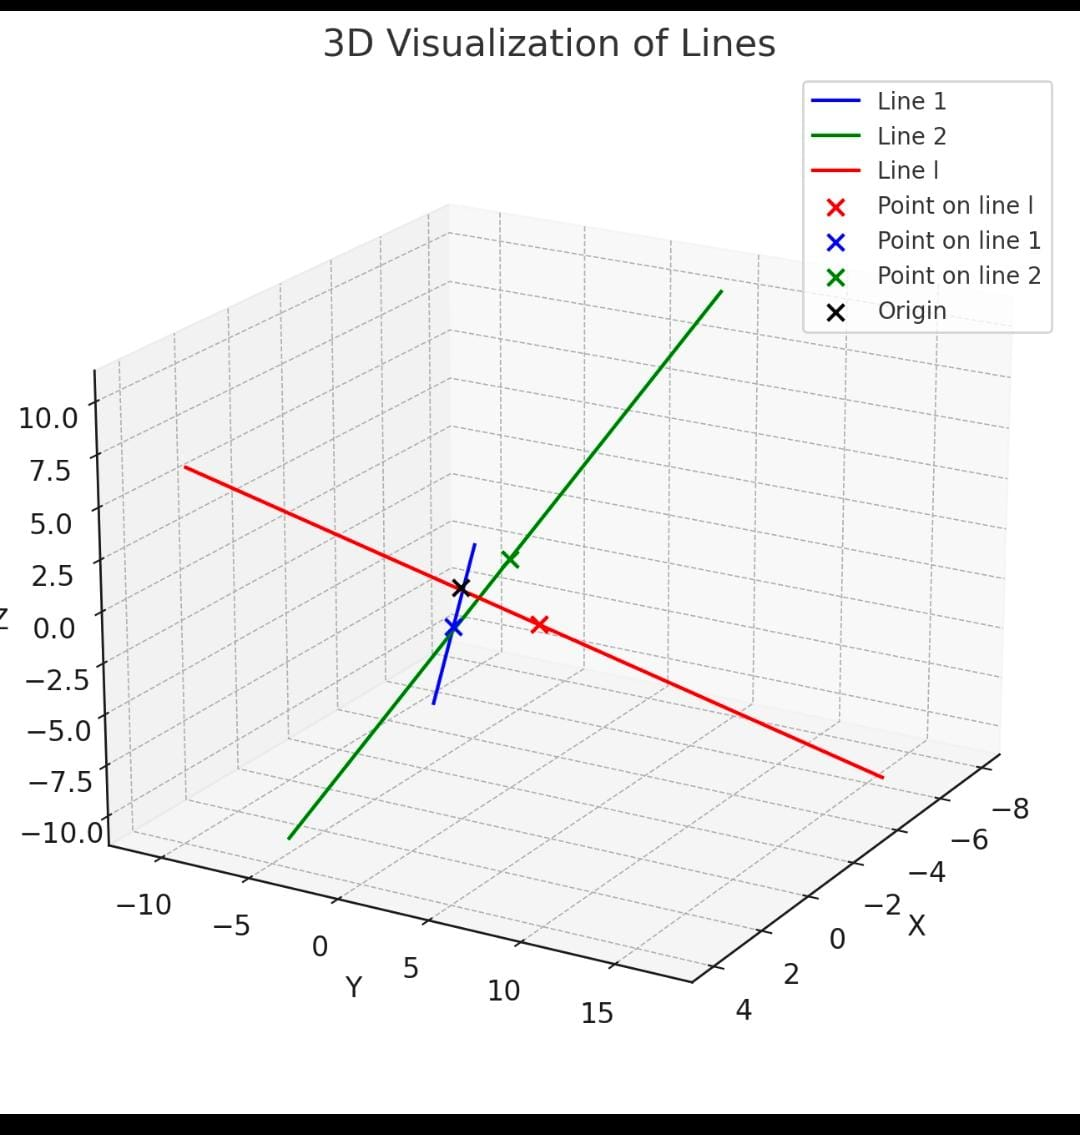
\includegraphics[width=0.65\textwidth]{matgeo-4.8.15.jpeg}
    \caption{}
    \label{fig:triangle5cm}
\end{figure}
\end{frame}

\end{document}
